% fancytikzposter.tex, version 2.1
% Original template created by Elena Botoeva [botoeva@inf.unibz.it], June 2012
% 
% This file is distributed under the Creative Commons Attribution-NonCommercial 2.0
% Generic (CC BY-NC 2.0) license
% http://creativecommons.org/licenses/by-nc/2.0/ 


\documentclass{a0poster}

\usepackage{fancytikzposter} 


%%%%% --------- Change here if you want ---------- %%%%%
%% margin for the geometry package, must be changed before using the geometry package
%% default value is 4cm
% \setmargin{4}

%% the space between the blocks
%% default value is 2cm
% \setblockspacing{2}

%% the height of the title stripe in block nodes, decrease it to save space
%% default value is 3cm
% \setblocktitleheight{3}

%% the number of columns in the poster, possible values 2,3
%% default value is 2
% \setcolumnnumber{3}

%% the space between two or more groups of authors from different institutions
%% used in \maketitle
% \setinstituteshift{10}

%% which template to use
%% N1 simple, standard look, with a colored background and gray boxes
%% N2 board with nodes
%% N3 another standard look
%% N4 envelope-like look
%% N5 with a wave-like head, original idea taken from
%%%% http://fc09.deviantart.net/fs71/f/2010/322/1/1/scientific_poster_by_nabuy-d333ria.jpg
\usetemplate{2}

%% components of the templates
%% (the maximal possible numbers are mentioned as the parameters)
% \usecolortemplate{4}
% \usebackgroundtemplate{5}
% \usetitletemplate{2}
% \useblocknodetemplate{5}
% \useplainblocktemplate{4}
% \useinnerblocktemplate{2}


%% the height of the head drawing on top 
%% applicable to templates N3, 4 and 5
% \setheaddrawingheight{14}


%% change the basic colors
%\definecolor{myblue}{HTML}{008888} 
%\setfirstcolor{myblue}% default 116699
%\setsecondcolor{gray!80!}% default CCCCCC
%\setthirdcolor{red!80!black}% default 991111

%% change the more specific colors
% \setbackgrounddarkcolor{colorone!70!black}
% \setbackgroundlightcolor{colorone!70!}
% \settitletextcolor{textcolor}
% \settitlefillcolor{white}
% \settitledrawcolor{colortwo}
% \setblocktextcolor{textcolor}
% \setblockfillcolor{white}
% \setblocktitletextcolor{colorone}
% \setblocktitlefillcolor{colortwo} %the color of the border
% \setplainblocktextcolor{textcolor}
% \setplainblockfillcolor{colorthree!40!}
% \setplainblocktitletextcolor{textcolor}
% \setplainblocktitlefillcolor{colorthree!60!}
% \setinnerblocktextcolor{textcolor}
% \setinnerblockfillcolor{white}
% \setinnerblocktitletextcolor{white}
% \setinnerblocktitlefillcolor{colorthree}




%%% size of the document and the margins
%% A0
% \usepackage[margin=\margin cm, paperwidth=118.9cm, paperheight=84.1cm]{geometry} 
\usepackage[margin=\margin cm, paperwidth=84.1cm, paperheight=118.9cm]{geometry}
%% B1
% \usepackage[margin=\margin cm, paperwidth=70cm, paperheight=100cm]{geometry}



%% changing the fonts
\usepackage{cmbright}
%\usepackage[default]{cantarell}
%\usepackage{avant}
%\usepackage[math]{iwona}
\usepackage[math]{kurier}
\usepackage[T1]{fontenc}


%% add your packages here
\usepackage{hyperref}
\usepackage[utf8]{inputenc} % slovenski znaki
\usepackage[slovene]{babel} % slovenski formati
\usetikzlibrary{shapes,arrows}

\title{Letter classification}
\author{Rok Koleša, Domen Kren, Darko Janković\\
  Faculty of Computer and Information science, University of Ljubljana
}


\begin{document}

%%%%% ---------- the background picture ---------- %%%%%
%% to change it modify the macro \BackgroundPicture
\ClearShipoutPicture
\AddToShipoutPicture{\BackgroundPicture}

\noindent % to have the picture right in the center
\begin{tikzpicture}
  \initializesizeandshifts
  % \setxshift{15}
  % \setyshift{2}


  %% the title block, #1 - shift, the default value is (0,0), #2 - width, #3 - scale
  %% the alias of the title block is `title', so we can refer to its boundaries later
  \ifthenelse{\equal{\template}{1}}{ 
    \titleblock{47}{1}
  }{
    \titleblock{47}{1.5}
  }

  %% a logo can be added to the title block
  %% #1 - anchor relative to the title block, #2 - shift, #3 - width, #3 - file name
  % \ifthenelse{\equal{\template}{2}}{ 
  %   \addlogo[south west]{(2,0)}{6cm}{unibz_b.png}
  % }{
  %   \addlogo[south west]{(2,0)}{6cm}{unibz_w.png}
  % }


  %% a block node, with the specified position (optional), title and the content
  %% #1 - where (optional), #2 - title, #3 - text
  %%%%%%%%%% ------------------------------------------ %%%%%%%%%%
  \blocknode%
  {Problem}%
  {Determine which capital letter is represented by given simplicial complex from the set of 12 letters of Slovenian alphabet. Simplicial complex is represented with a list of edges which consist of pairs of start and end points. Each point is given by a pair of coordinates.
  
  
  Start with the following document:

    \coloredbox{colorthree!50!}{
      \textbackslash documentclass\{a0poster\}\\
      \textbackslash usepackage\{fancytikzposter\} \% here most of the things are
      defined \\

      \% change parameters only after this line\\

      \textbackslash usepackage{\small[margin=\textbackslash margin \ cm,
        paperwidth=84.1cm, paperheight=118.9cm]\{ geometry\}} \\

      \textbackslash title\{Title\}\\
      \textbackslash author\{Author\textbackslash\textbackslash
      Institution\textbackslash\textbackslash
      \textbackslash texttt\{email\}\}\\
      \textbackslash begin\{document\}\\
      \textbackslash AddToShipoutPicture\{\textbackslash BackgroundPicture\}\\


      \textbackslash noindent \\
      \textbackslash begin\{tikzpicture\} \\
      \textbackslash initializesizeandshifts \\

      \textbackslash titleblock\{50\}\{1\}\\
      \textbackslash blocknode\{Block Title\}\{Block Content\}\\
      \textbackslash startsecondcolumn\\
      \textbackslash blocknode\{Block Title 2\}\{Block Content 2\}\\
      \textbackslash end\{tikzpicture\}\\
      \textbackslash end\{document\}
    }
  }


  %% a callout block
  %% #1 - rotate angle (optional), #2 - from, #3 - where, #4 - width, #5 - text
  %%%%%%%%%% ------------------------------------------ %%%%%%%%%%
  \calloutblock{($(box.center)+(-2,-8)$)}
  {($(box.center)+(10,-1)$)}
  {19cm}
  {\small
    Macro for creating a block node:
    \begin{itemize}
    \item[] \textbackslash blocknode\{Block Title\}\{Block Content\}
    \end{itemize}
    Macro \textbackslash blocknode has three parameters. The first one is
    optional and it is the position of the block. The first block will be
    automatically placed to (\$(firstrow)-(xshift)-(yshift)\$), which is the
    left corner below the title block. In most of the templates, (firstrow) is
    set to (title.south), where \emph{title} is the alias for the title
    block. Each subsequent block is automatically placed to
    [(\$(box.south)-(yshift)\$)], i.e., below the previous block aliased
    \emph{box}.  You can also use an explicit parameter, e.g., $(-10,30)$ (note
    that (0,0) is the center of the poster). The second parameter is the title
    of the block. Finally, the last parameter is the  actual content. 
  }




  %% by default, the position of the new block node is right below the previous
  %% block node, stored in (currenty)
  %% box is the alias of the previous block, so we can refer to its boundaries

  %%%%%%%%%% ------------------------------------------ %%%%%%%%%%
  \blocknode{Results}%
  {With described method we were able to successfully classify input data.  

  }
  

  %%%%%%%%%% ------------------------------------------ %%%%%%%%%%
  \blocknodew[($(currenty)-(3.5,0)$)]{30}{Variable Width Block Nodes} %
  { You can also create blocks of arbitrary width
    \begin{itemize}
    \item[] \textbackslash blocknodew[coordinate]\{Block width\}\{Block Title\}%
      \{Block Content\}
    \end{itemize} 
    % 
    In this case it is better to specify coordinate manually if you want to have
    blocks aligned vertically. \\

    Note that (xshift) and (yshift) are coordinates created in macro
    \textbackslash initializesizeandshifts, and they allow to have relative
    positioning of block nodes in an automatic fashion. If you want to define
    your own shifts, set new values for (xshift) and (yshift) using commands
    \textbackslash setxshift and \textbackslash setyshift.\\

    Also, it might be useful to know the y-coordinate of the south border of the
    previous block. You can retrieve it by using the command
    \begin{itemize}
    \item[] \textbackslash getcurrentrow\{box\} or \textbackslash getcurrentrow\{note\}
    \end{itemize}
    This coordinate will be stored in (currentrow), which can be used to
    specify the location of the next block node.
  }


  %%%%%%%%%% ------------------------------------------ %%%%%%%%%%
  \plainblock[5]{($(currenty)+(4,2)$)}{35}{fancyTikZposter template} %
  {
    
    \vspace{0.3cm}
    It is a template for scientific posters based on a0poster and TikZ
    only. The current version contains five (plus one) different templates (see my
    posters
    % 
    \href{http://www.inf.unibz.it/~ebotoeva/presentations/abcrs-KR-12-poster.pdf}{%
      \underline{here}} and
    % 
    \href{http://www.inf.unibz.it/~ebotoeva/presentations/boto-RR-12-poster.pdf}{%
      \underline{here}}). The sources of this pdf file can be found
    \href{http://www.inf.unibz.it/~ebotoeva/tikz/tikzposter_sources.zip}{\underline{here}}.}

  


  %%%%%%%%%%%%% NEW COLUMN %%%%%%%%%%%%%%% 
  \startsecondcolumn 

  %%%%%%%%%% ------------------------------------------ %%%%%%%%%%
  \blocknode%
  {Solution}%
  {
Solution

As seen in our goal specification, we tackled this problem of letter classification with persistent homology. 
The main idea of our solution is looking at different parts of objects and computing their homologies. The 
algorithm is divided into three parts:

1.) First, let us parse the input. All we need is a set of points that are part of the object we want to classify. The
only problem that can arise, comes from the distribution of the points. If they are all in one place or to scarce, we
will not be able to get good results. We want an even distribution with lots of points.

2.) We slowly "sink" our letter. After sorting our input points we cut the letter by layers. After that we compute 
homologies for each of those. 

For the computations, we use the VietorisRips filter and check the intervals of our 
simplexes. In this case, we take the infinite ones. With that we can get the number of pieces and cycles in our complex.
We have to be a little careful with how we chose the maximum radius value, for the VietorisRips algorithm. With some
trial and error we decided on 10% of the full object size. With that we remove most of errors. 

Now let us return to the "sinking". For example, lets break letter "A" into 6 pieces. First, we take the lowest piece and 
get its 0. and 1. dimension homologies. The next step is the lowest two pieces, then three, ... What we get in the end is 
a diagram with numbers corresponding to the number of pieces and cycles for every part of the letter.

3.) The last thing we need to do is classify the letter. Based on some observations we made a decision tree, which "sinks"
the given letter in many directions and based on the observations chooses the correct paths. For example, in the first
stage we look at the number of cycles in the letter. Based on that information we can already separate "B" from the others, as
it is the only one with 2. With this information can also separate "A" and "D" from all the others. Every group of potential
candidates can be separated with different information(we "sink" top to bottom, left to right, 45degres angle, ...) until we
are left with only one candidate in each node. This candidate corresponds to our original letter so we return it. 

  
    \begin{tikzfigure}[A shaded circle]
     \begin{tikzpicture}
        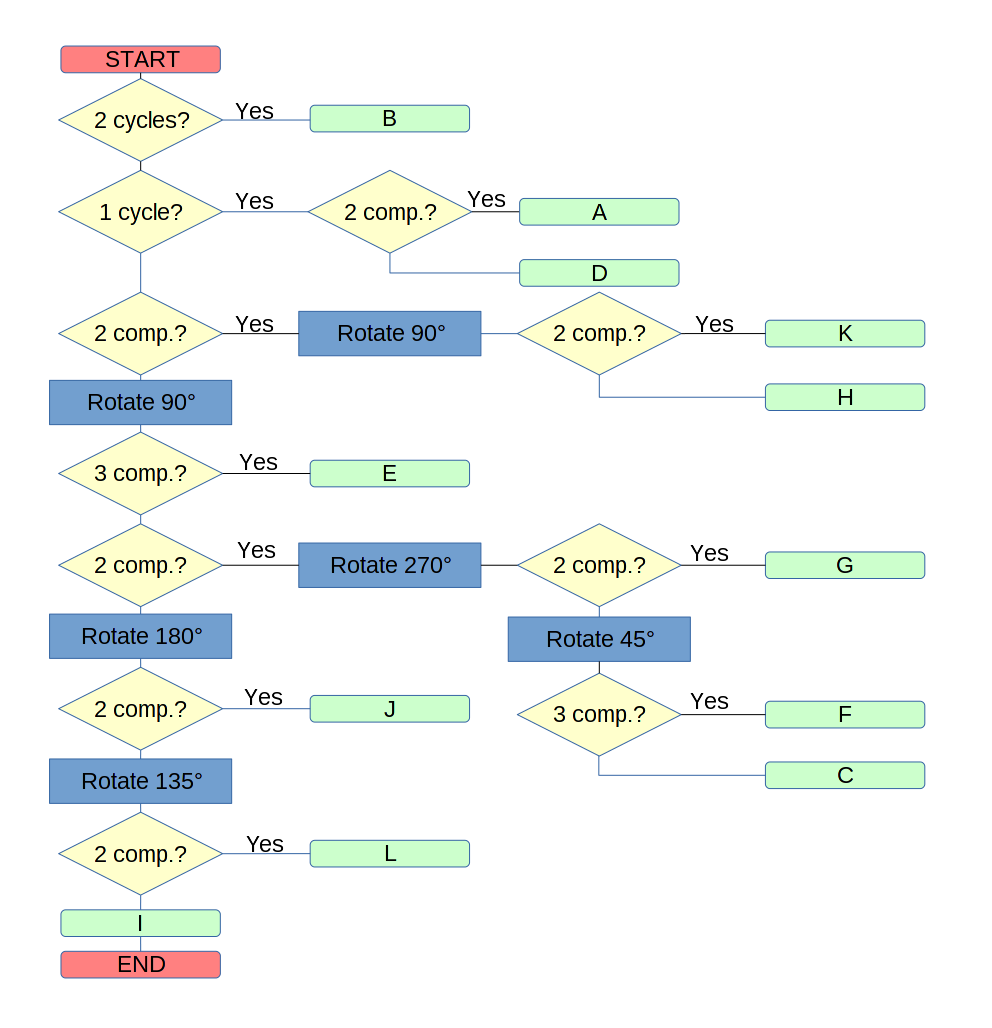
\includegraphics[scale=1]{../images/DecisionTree.png}
      \end{tikzpicture}
    \end{tikzfigure}
    
    
  }


  
  %%%%%%%%%% ------------------------------------------ %%%%%%%%%%
  \blocknode{Useful Macro Within Block Nodes}%
  {There are three types of colored boxes/blocks that you can use inside block
    nodes to highlight information. \\
    
    \begin{tabular}[t]{ll}
      \begin{minipage}{0.5\linewidth}
        \innerblock{Theorem} {Statement}
      \end{minipage}
      & 
      \textbackslash innerblock\{Theorem\}\{Statement\}\\

      \begin{minipage}{0.5\linewidth}
        \innerblockplain[colorone!80!]{Text}
      \end{minipage}
      &
      \textbackslash innerblockplain[colorone!80!]\{Text\}\\ 

      \begin{minipage}{0.5\linewidth}
        \coloredbox{colorthree!50!}{Text}
      \end{minipage}
      &
      \textbackslash coloredbox\{colorthree!50!\}\{Text\}
    \end{tabular}

    \vspace{0.5cm}
    The default figure environment does not work within a tikzpicture. I created
    a new figure environment that can be used instead, based on the code sent by
    Stephan Thober.
    \begin{itemize}
    \item[] \textbackslash begin\{tikzfigure\}[Caption]\\
      \ldots\\
      \textbackslash end\{tikzfigure\}
    \end{itemize} 
    % 

    \begin{tikzfigure}[A shaded circle]
      \begin{tikzpicture}
        \draw[draw=none,inner color=colorthree, outer color=colorone] (0,0) circle (2cm);
      \end{tikzpicture}
    \end{tikzfigure}
    
  }


  %%%%%%%%%% ------------------------------------------ %%%%%%%%%%
  \calloutblock{($(box.south east)-(8,-2)$)}
  {($(box.south east)-(16,2)$)}
  {30cm}
  {
    There are also callout blocks that allow for a more interesting layout of the
    poster. 
    \begin{itemize}
    \item[] \textbackslash calloutblock[rotate angle]\{from
      coordinate\}\{coordinate\}\{Block Width\}\{Block Content\} 
    \end{itemize}
    The alias for such blocks is \emph{note}.
  }


  %% to place the next node centered vertically in the second column, we can
  %% obtain the y-coordinate of the previous node using macro
  %% \getcurrentrow{note}, where note is the alias of the callout node, and
  %% then specify the coordinate of the next node using coordinate (currentrow)
  \getcurrentrow{note}



  %% a plain block
  %% #1 - rotate angle (optional), #2 - where, #3 - width, #4 - title, #5 - text
  %%%%%%%%%% ------------------------------------------ %%%%%%%%%%
  \plainblock{($(currentrow)+(xshift)-(yshift)$)}%[($(currenty)+(0,10)$)]%
  {32}{Plain blocks} %
  {These blocks are similar to callout blocks. They allow for specifying the
    title of the block.
    \begin{itemize}
    \item[] \textbackslash plainblock[rotate angle]\{coordinate\}\{Block Width\}\{Block
      Title\}\{Block Content\} 
    \end{itemize}
  }


 
  %% the coordinate (currenty) is used in the default placing of the next blocknode
 \getcurrentrow{note}
 \coordinate (currenty) at ($(currentrow)+(xshift)-(yshift)$);



   %%%%%%%%%%%%% NEW COLUMN %%%%%%%%%%%%%%% 
  %% (if column number is 3)
  \startthirdcolumn

  %%%%%%%%%% ------------------------------------------ %%%%%%%%%%
  \blocknode {Personalizing the Poster}%
  {It is possible to adjust the layout of the poster. To impose your own
    setting, you can use these macros:
    \begin{itemize}
    \item Macros for changing sizes
      \begin{itemize}
      \item[] \textbackslash setmargin\{4\},
        %% the height of the head drawing on top
        %% applicable to templates N2 and 4
        \textbackslash setheaddrawingheight\{14\},
        %% the space between two or more groups of authors from different
        %% institutions
        %% used in \maketitle
        \textbackslash setinstituteshift\{10\},\\
        %% the space between the blocks
        %% default value is 2cm
        \textbackslash setblockspacing\{2\},
        %% the height of the title stripe in block nodes, decrease it to save space
        %% default value is 3cm
        \textbackslash setblocktitleheight\{3\}
      \end{itemize}

    \item Other structural macros
      \begin{itemize}
      \item[]  %% the number of columns in the poster, possible values 2,3
        %% default value is 2
        \textbackslash setcolumnnumber\{3\},
        %% which template to use 
        %% N1 simple, standard look, with a colored background and gray boxes
        %% N2 board with nodes
        %% N3 another standard look
        %% N4 envelope like look
        %% N5 with a wave-like head, original idea taken from
        %%%% http://fc09.deviantart.net/fs71/f/2010/322/1/1/scientific_poster_by_nabuy-d333ria.jpg
        %% N6 experimental, oriental style, largely based on template N3
        \textbackslash usetemplate\{6\},\\
        \textbackslash usecolortemplate\{4\},
        \textbackslash usebackgroundtemplate\{5\},
        \textbackslash usetitletemplate\{2\},\\
        \textbackslash useblocknodetemplate\{5\},
        \textbackslash useinnerblocktemplate\{3\},
        \textbackslash useplainblocktemplate\{4\}

      \end{itemize}

    \item Macro for adding logos to the title block
      \begin{itemize}
      \item[] \textbackslash addlogo[south west]\{(0,0)\}\{6cm\}\{filename\}
      \end{itemize}

    \item Macros for the basic colors
      \begin{itemize}
      \item[] \textbackslash setfirstcolor\{green!70!\}, % default 116699
        \textbackslash setsecondcolor\{gray!80!\}, % default CCCCCC
        \textbackslash setthirdcolor\{red!80!black\}% default 991111
      \end{itemize}

    \item Macros for specific colors:
      \begin{itemize}
      \item[] \textbackslash setbackgrounddarkcolor\{colorone!70!black\},
        \textbackslash setbackgroundlightcolor\{{\small colorone!70!}\},\\
        \textbackslash settitletextcolor\{textcolor\},
        \textbackslash settitlefillcolor\{white\},
        \textbackslash settitledrawcolor\{colortwo\},\\
        \textbackslash setblocktextcolor\{textcolor\},
        \textbackslash setblockfillcolor\{white\},\\
        \textbackslash setblocktitletextcolor\{colorone\},
        \textbackslash setblocktitlefillcolor\{colortwo\}, \\
        \textbackslash setplainblocktextcolor\{textcolor\},
        \textbackslash setplainblockfillcolor\{colorthree!40\},\\
        \textbackslash setplainblocktitletextcolor\{textcolor\},
        \textbackslash setplainblocktitlefillcolor\{colorthree!60\}, \\
        \textbackslash setinnerblocktextcolor\{textcolor\},
        \textbackslash setinnerblockfillcolor\{white\},\\
        \textbackslash setinnerblocktitletextcolor\{white\},
        \textbackslash setinnerblocktitlefillcolor\{colorthree\},
      \end{itemize}
    \end{itemize}
  }



\end{tikzpicture}


\end{document}




